
\chapter{Model Overview}
\label{ch:model-overview}

\section{Environment}

Explain how the environment is represented.

\subsection{Nodes}

The fundamental entity to represent the environment the \emph{Node} interface. A node can be seen as an infinitesimal piece of the environment. By linking nodes together it is possible to create complex network of objects that will describe the space where agents can navigate.

The \emph{Node} interface does not specify how these connections need to be made and how many neighbours each node has. This gives a great degree of freedom to users, for example it is ease to declare different types of nodes, that can describe different types of environment. For example, the \emph{BasicNode} class is used to describe two dimensional environments, as we will see later on. A three dimensional environment could be easily described as well though, by implementing the \emph{Node} interface with 6 neighbours, one in each direction - north, south, east, west, above and bellow, agents would be able to navigate through nodes in three different axis.

(((add and describe methods for neighbours)))

Each node has an unique string that is used to identify them. The method \emph{getId()} returns this string, which should be unique. Note that the \emph{Node} interface does not have any instrument to guarantee that nodes have unique identifiers, it is up to the users of the interface to guarantee that nodes do not have duplicated identifiers. 

Nodes also have a list of agents (see section \ref{sec:agents}), this is the list of agents that are currently in the node. The node interface provides the necessary methods to operate upon the agents, these are:

\begin{itemize}
  \item void addAgent(Agent): Verify if the agent can be added to the node, if yes, adds the agent to the node, if not ignores..
  \item List<Agent> getAgents(): Return the list of agents currently in the node
  \item void addAgentStartingHere(Agent): This method is used to place agents into the environment. \emph{addAgent(Agent)} method might have to check for few conditions before allowing the agent into the node. Agents that are starting their lifecycle could fail to pass this conditions. So this method is provided, and it does nothing else but add the agent to the node.
\end{itemize}

For the agents list is published, that is, it is accessible to many threads, any implementation of the \emph{Node} interface must be thread-safe.

Agents are able to indirectly communicate to each other through the use of communication stimuli (see subsection \ref{subsec:comm-stimulus}) that they add or manipulate existing ones in their environment.

The \emph{Node} interface specifies the following methods to manipulate communication stimuli:

\begin{itemize}
  \item List<CommunicationStimulus> getCommunicationStimuli(): returns a list of all communication stimulus present in the node
  
  \item void addCommunicationStimulus(CommunicationStimulus): add a new communication stimulus to the node.
  
  \item CommunicationStimulus getCommunicationStimulus (CommunicationStimulusType): returns a communication stimulus of the type specified, if one is present in the list.
\end{itemize}

Each communication stimulus has a type. The type determines which proprieties are present for a stimulus. The \emph{Node} interface enforces no limitation on having more than one stimulus of the same type in the communication stimulus list. There will be cases that makes no sense in having two stimulus of the same tape in the list. For example, imagine that we have two ants that deposit chemical substances (pheromones) in the environment to communicate to each other. Let say the first ant deposit 0.1 and the second ant another 0.1 of the same pheromone. As far the other ants are concerned the total of that pheromone in that node is 0.2, it does not matter to know when they where deposited and by which ant. In this case it makes sense to have only one type of communication stimulus in the list to represent that type of pheromone, each ant can update that stimulus if necessary. That is exactly what the \emph{ChemicalStimulusType} class (see  subsection \ref{subsec:chemical-stimulus}) and its implementations do. There could be cases that having two stimulus of the same type in the list is valid, for instance when a stimulus expires after some time or when it is necessary to know the agent that issued a particular stimulus

In case more than one communication stimulus of the same type is allowed in the list, the \emph{Node} interface does not specifies which one should be returned when the method \emph{getCommunicationStimulus(CommunicationStimulusType)} is called. It is up to the user to decide how to handle the request.

\subsubsection{BasicNode Class}

The \emph{BasicNode} class is the reference implementation of the \emph{Node} interface for a 2 dimensional space, with nodes connected to 4 neighbours.

It is a pseudo-thread-safe class. The methods \emph{getNeighbour(Direction)}, \emph{getNeighbour(Direction, Node)} and \emph{setNeighbours(Direction, Node)} do not make use of synchronisation mechanisms that would guarantee thread-safety. The reason for that is that this methods are exhaustively used during simulations, and the lack of synchronisation mechanisms here remove any overhead introduced by them. It is safe to not use synchronisation in these methods as long as the environment does not change during the simulations. Note that this is documented in the code by the use of the annotations \emph{@PseudoThreadSafe} and \emph{@ThreadSafetyBreaker}, see subsection \ref{subsec:doc-annotations} for more details.

Each basic node can have a maximum of four neighbours, one in each direction defined by the Direction enumeration (see \ref{subsec:direction-enum}): North, East, South and West.

The \emph{BasicNode} implementation of \emph{getCommunicationStimulus} method returns the first stimulus of the requested type found in the list. If none is found, \emph{null} is returned.

\subsubsection{PheromoneNode Class}

The \emph{PheromoneNode} class is a specialisation of the \emph{BasicNode}, exclusive for ant simulations. In addition of everything present in the super class, it declares two new methods that come handy when dealing with chemical communication stimuli (see subsection \ref{subsec:chemical-stimulus}):

\begin{itemize}
  \item ChemicalCommStimulus getCommunicationStimulus (ChemicalCommStimulusType): This method returns a chemical communication stimulus of the requested type if any is present in the stimuli list. If there are more than one stimulus of the same type, the first one found is returned. If none is present, it created a new chemical stimulus of that type, adds it to the stimuli list and returns the new created stimulus.

  \item void increaseStimulusIntensity (ChemicalCommStimulus, double): Increment the intensity of the chemical stimulus of the requested type. If no stimulus of the type is present, it adds one to the list and increment by the specified amount.
\end{itemize}

The first method is just an overload of the generic \emph{getCommunicationStimulust(CommunicationStimulustType)} method from \emph{Node} interface. Clients do not necessarily need to use this method when creating ants experiments, it is just a shortcut to be used in order to avoid casting.

The same is valid for the second method. Agents could increase a stimulus intensity directly, but buy using the \emph{increaseStimulusIntensity} method clients take advantage of existing infrastructure, simplifying their code.

\subsection {Communication}
\label{subsec:comm-stimulus}

\subsection{Communication Stimulus}

Agents have their own lifecycle, their own intentions and goals. Communication is a vital part of the process of achieving their goals, for in most cases agents cannot deal with all challenges imposed by the problems they are trying to solve by themselves.

There are plenty of examples that illustrates that around us. If someone is going to build a house, they most certainly will need help do be able to do it. Not only physical help, they will need another people's skills. (((need to find another example in nature that are not ants or bees))).

The \emph{CommunicationStimulus} interface is an abstraction of any communication interaction. Implementations of the interface are required to implement only one public method:

\begin{itemize}
  \item CommunicationStimulusType getType(): Returns what type of communication stimulus the object is.
\end{itemize}

The class \emph{BasicCommunicationStimulus} offer a simple reference implementation of the \emph{CommunicationStimulus} interface and is the perfect class to extend when creating complex communication stimuli.

\subsection{Communication Stimulus Type}

We have many ways to communicate, we can talk to other people, we can write them an e-mail or use sign language to transmit any information we find useful to transmit. Everyone knows that a dog barks, what information exactly it is transmitting we are not able to decode yet, and maybe we never will. Anyway some information is being transmitted in the process. Dogs also use another way to communicate. They urinate in order to mark territory.

The \emph{CommunicationStimulusType} interface is an high level abstraction of a specific way to communicate. As such it formalises only o public method:

\begin{itemize}
  \item String getName(): Returns the name of the type of communication stimulus.
\end{itemize}

By extending this interface users can formalise different types of communication. Adding extra parameters necessary to their specific communication types.

Implementations of \emph{CommunicationStimulusType}, and any of its specialisations, must be singletons (see section XX) in order to save computational resources.

\subsubsection{Chemical Communication Stimulus}
\label{subsec:chemical-stimulus}

As seen in section \ref{sec:ant-comm}, ants use pheromone as a way to communicate indirectly to fellow ants of the same nest. The interface \emph{ChemicalCommStimulusType} extends \emph{CommunicationStimulsType} to formalise pheromone as a type of communication. It declares two public methods:

\begin{itemize}
  \item double getDecayFactor(): Returns the decay factor of the chemical type. 
  \item int getRadius(): Returns the radius of action of the pheromone.
\end{itemize}

The class \emph{ChemicalCommStimulus} is the base implementation for using this new communication type. It adds a new propriety to the communication: \emph{intensity}. This new field is a double that represents the intensity of the pheromone in that communication stimulus. The class is thread-safe, and \emph{intensity} is guarded by the class.

The key methods of the class are:

\begin{itemize}
  \item void synchronised increaseIntensity(double): Increases the intensity of the chemical stimulus by the amount passed as parameter.
  
  \item void synchronised decayIntensity(): Decays the intensity of the stimulus depending on its type.
\end{itemize}

It is important to note that \emph{ChemicalCommStimulus} limits the maximum amount of intensity to 1.0. If an agent tries to increment a stimulus that is already 1.0 in intensity, the request is ignored.
Another noteworthy point is how \emph{ChemicalCommStimulus} implements the intensity decay. It uses the following:

\begin{equation}
intensity_{new} = intensity * (1 - decayFactor)
\end{equation}

The \emph{decayFactor} parameter above comes from the chemical communication type declared by the users. See section \ref{subsec:forage-stimulus} for an example of a type implementation.

\subsubsection {Forage Communication Stimulus}
\label{subsec:forage-stimulus}

This communications stimulus type is used by ants when foraging. Is is deposited whether when ants are searching for food or going back to the nest caring food. The amount deposited should be higher if ants are caring food and going back to their nest. This is a form of positive feedback (see \ref{subsec:feedback}).

One should expect for this type of pheromone to have a small decay factor, as it needs to have a long lasting effect on the agents in order to them to be able to collect food from sources far from the nest. As well as short action radius, for large radius would 'confuse' agents within the trail.

The enumeration \emph{ForageStimulusType} is an extension of \emph{ChemicalCommStimulusType} and declares this stimulus type.

\subsubsection {Warning Communication Stimulus}

\emph{WarningStimulusType} is also an extension of \emph{ChemicalCommStimulusType}, it represents a whole different type of information though. It is an analogy to the pheromone laid by soldier ants to warn their fellows of any danger around. Different type of agents react differently to the same communication stimulus (see \ref{sec:agent-types}), but one would expect this type of stimulus to have a high decay factor and a large radius of action. The former will avoid too many soldier of being recruited to attack a predator for instance. The latter would allow the stimulus to reach a larger number of ants around the danger faster.

\subsection{Environment Package}

\begin{figure}[H]
  \centering
  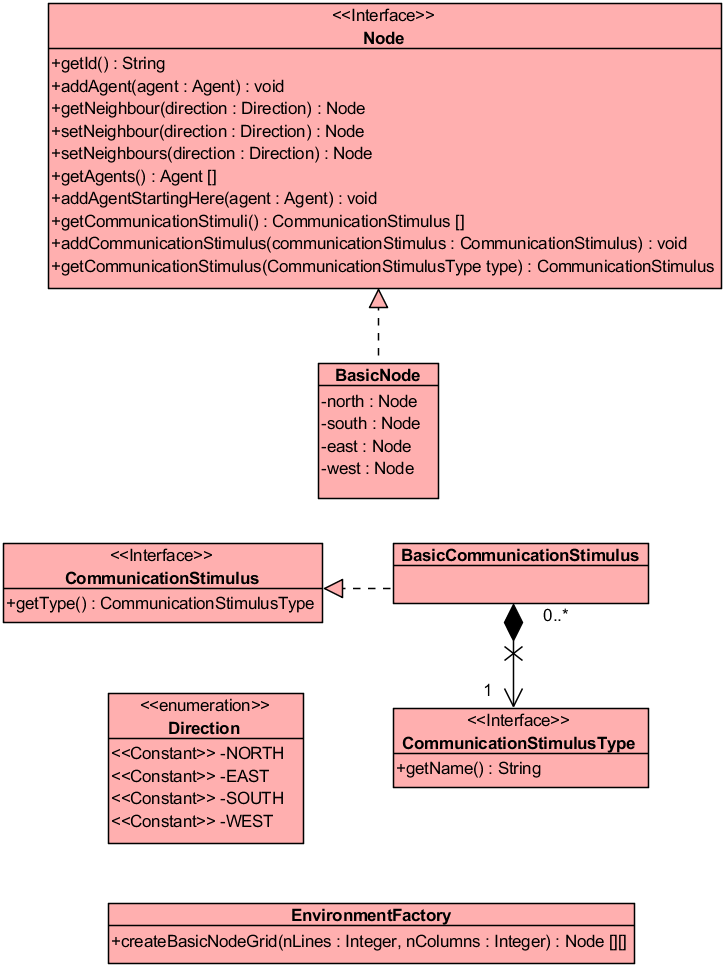
\includegraphics[width=1.0\linewidth]{gfx/uml-env-package.png}
  \caption{The generic model package}
  \label{fig:gen-env-package}
\end{figure}

\section {Agents}
\label{sec:agents}

To enable the agents defined by the model to enjoy the properties that define agents in general it is critical that they have their own lifecycle, and the most flexible way to achieve that is if each agent is run in an isolated thread in one of the available CPUs of the machine running the simulation. This is guaranteed by the \emph{AbstractAgent} which implements the \emph{Callable} interface (see section \ref{subsec:threads-task-exec} for more details).  

The abstraction of any agent is the \emph{Agent} interface though. It formalises the basic API that is available to any agent in the model. The most relevant are:

\begin{itemize}
  \item String getId(): Each agent must have an unique identifier string to be used for identification. This method returns it. Note that is up to the user to make sure this string is unique.
  
  \item AgentType getAgentType(): Returns the type associated with the agent.
  
  \item void setCurrentNode(Node): Places the agent in a specific node of the environment.
\end{itemize}

There are another methods that are related with tracking the nodes the agent has been in the environment during the simulation, more information on these methods can be found in the appendix \ref{chapter:model-code}.

The \emph{AbstractAgent} is the base abstract implementation of the \emph{Agent} interface. It implements all the public methods declared by the interface, plus declares the implementation of the \emph{Callable} interface, returning the type \emph{Void}, which is a convention to tell the compiler that no value is expected to be returned. By being abstract and declaring the implementation of \emph{Callable}, the class effectively forces any concrete specialisation class to implement the methods that define a task in Java, therefore allowing any agent to be executed in an isolated thread.

\subsection{Task Agents}

Explain that a specialisation of the Agent interface is proposed to create agents that are capable of executing tasks.

\subsection{Agent Types}
\label{sec:agent-types}

Explain what are agents types and why they are necessary. relate with cases in nature.

\section {Tasks}

Tasks are a unit of specialised work. Agents types have a list of tasks that a particular type is able to execute. Explain how agents can switch between tasks depending on the context.
